\section{ تعمیم یادگیری‌ها به ابعاد بالاتر}
\begin{frame}[standout]
ماشین تانسور پشتیبان 
\\
\small{ تعمیم ماشین بردار پشتیبان}
\end{frame}
\begin{frame}{STM}
\small{
ماشین بردار پشتیبان از بهینه‌سازی استفاده می‌کند و  هدف آن پیدا کردن مرزهای جداسازی بهینه است. این مرز‌های بهینه با کمینه کردن خطا میان تمام مرز‌های ممکن تخمین زده شده توسط نمونه‌ها بدست می‌آید. تابع تصمیم ماشین بردار پشتیبان کلاسیک را می‌توان به صورت 
\[y(\mathrm{a}) = sign(w^\trans a + b)\]
نوشت. 
$\mathrm{a}\in \mathbb{R}^{L \times 1}$
بردار بدون برچسب ورودی، 
$y \in \{ -1,+1 \}$ برچسب حدس زده شده و
$w \in \mathbb{R}^{L \times 1}$
ماتریس تصویر است. 
}
\end{frame}
\begin{frame}{STM}
\small{
پارامتر‌های این مدل را می‌توان با حل کردن بهینه‌سازی زیر بدست آورد: 
\begin{align*}
\underset{w,b,\xi}{\min} &f(w,b,\xi) =  \frac{1}{2}\norm{w}^2 + c\sum_{i=1}^{N} \xi_i  \notag \\  
\text{\lr{s.t.}}\hspace{3mm} &y_i \left[ w^\trans \mathrm{a}_i + b \right] \geq 1 - \xi_i,\hspace{2mm}\xi_i \geq 0, \hspace{3mm} 1\leq i\leq N
\end{align*}


هدف اصلی  
\textbf{ماشین تانسور پشتیبان}
یافتن ابرصفحاتی است که داده‌های تانسوری را با توجّه به نمونه‌های آموزشی از هم جدا کند. تابع تصمیم‌گیری چندخطی برای ماشین تانسور پشتیبان،
 داده‌ی تانسوری بدون برچسب ورودی 
 \linebreak 
$\mathcal{A} \in \mathbb{R}^{I_1 \times I_2 \times \cdots I_N}$،
به صورت 
\begin{align*}
y(\mathcal{A}) = sgn \left(  \mathcal{A} \prod_{k=1}^{N} \times_k w_k + b \right)
\end{align*}
تعریف  می‌شود. که در آن 
$y \in \{ +1,-1 \}$،
$b$
است.
}
\end{frame}
\begin{frame}{STM}
\small{
	وزن‌های
$w_k$
 به صورت زیر محاسبه می‌شود: 
\begin{align}\label{STM_Primal}
\underset{w_k |_{k=1}^{N}}{\min} &f\left( w_k |_{k=1}^{N}, b, \xi\right) = \frac{1}{2} \|{ w_1 \circ w_2 \circ \cdots \circ w_N }\|^2 + c\sum_{i=1}^{N} \xi_i\\
\text{\lr{s.t.}}\hspace{3mm} & y_i \left[ \mathcal{A}_i \prod_{k=1}^{N} \times_k w_k + b \right] \geq 1 - \xi_i, 1\leq i\leq M , \hspace{3mm}\xi_i \geq 0 \notag
\end{align}

\pause
که در آن 
$w_k |_{k=1}^{N}$
 بیانگر وزن در حالت 
$k$ام
است. در این معادله، 
$\xi_i$
بردار متغیّر اسلک بوده و 
$c$
ضریب منظّم‌ساز برای کنترل خطا‌های طبقه‌بندی است. همچنین 
$M$
تعداد کلّ نمونه‌ها و 
$\mathcal{A}_i$ 
نشان‌دهنده‌ی 
$i$امین
تانسور داده‌های آموزشی است. 
}
\end{frame}
\begin{frame}{STM}
\small{
 	می‌توان از روش‌های 
	\textit{متناوب}
	برای پیدا کردن جوابی مناسب استفاده کرد. گرچه این روش‌ها تضمینی برای رسیدم به نقطه‌ی کمینه به ما نمی‌دهند اما ثابت شده که همواره به یک نقطه‌ی کمینه‌ی محلی خواهند رسید. پس از محاسبه‌ی 
	$w_j$ و
	$b$
	می‌توان ابرصفحه‌ی جداساز را با استفاده از رابطه‌ی زیر محاسبه کرد:
	
	\pause
	\begin{align*}
	\mathcal{A}\prod_{k=1}^{N} \times_k w_k + b = 0.
	\end{align*}
}
\end{frame}
\begin{frame}
\small{
	نمایی از جداسازی دودویی  به وسیله‌ی ماشین تانسور پشتیبان در فضای با ابعاد بالا 

}
	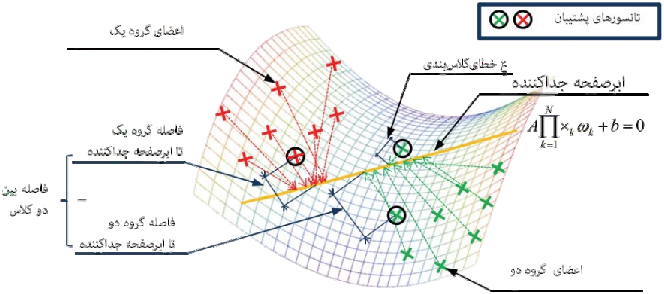
\includegraphics[width=1\textwidth]{img/ok/STM.pdf}

\end{frame}
\begin{frame}[standout]
Tensor Spectral Clustering
\end{frame}
\begin{frame}[standout]
Logistic Tensor Regression
\end{frame}
